\section{Growth laws and the price of a sound takeoff}\label{sec:scaling}

\subsection{Osgood takeoffs}

Theorems~\ref{thm:E} and~\ref{thm:F} take the costs $a_{n}$ as given. Growth models of an intelligence explosion produce them. The simplest such model, and the one behind most informal arguments, is the equation
\[
\frac{dI}{dt}=c\,I^{\alpha},\qquad c>0,\ \alpha>0,
\]
for a capability $I$ that speeds up its own improvement. Its solution from $I(0)=1$ reaches infinity at the finite time $\int_{1}^{\infty}dI/(cI^{\alpha})=1/(c(\alpha-1))$ when $\alpha>1$ and grows without blowing up when $\alpha\le1$; Osgood's criterion states the same for $dI/dt=f(I)$ with the integral of $1/f$ \cite{Osg98}.\footnote{W.~F. Osgood, \emph{Beweis der Existenz einer L\"osung der Differentialgleichung $dy/dx=f(x,y)$ ohne Hinzunahme der Cauchy--Lipschitzschen Bedingung}, Monatshefte f\"ur Mathematik und Physik 9 (1898), 331--345 \cite{Osg98}. The paper is about uniqueness; the blow-up criterion that bears Osgood's name is the elementary fact, implicit there, that a solution of $y'=f(y)$ with $f>0$ reaches infinity in the finite time $\int_{y_{0}}^{\infty}dy/f(y)$ exactly when the integral converges. For $f(y)=cy^{\alpha}$ the integral is $y_{0}^{1-\alpha}/(c(\alpha-1))$ for $\alpha>1$ and diverges for $\alpha\le1$.} To put a check on the curve one has to say what one improvement is. Two choices are natural.

\emph{Additive steps.} The $n$-th improvement raises the capability from $n$ to $n+1$ at the rate reached at its start, so it takes the time $g_{n}=1/(cn^{\alpha})$.

\emph{Multiplicative steps.} The $n$-th improvement multiplies the capability by a fixed factor $\lambda>1$, from $\lambda^{n-1}$ to $\lambda^{n}$, at the rate reached at its start, so it takes the time $g_{n}=(\lambda-1)\lambda^{n-1}/(c\lambda^{(n-1)\alpha})=\frac{\lambda-1}{c}\,q^{n-1}$ with $q=\lambda^{-(\alpha-1)}$.

In both cases we let the check of the $n$-th improvement cost a fixed fraction $\kappa>0$ of the time it took to make, $a_{n}=\kappa g_{n}$ per run, so that faster improvements are also faster to check. Write $G=\sum_{n}g_{n}$ for the unchecked takeoff time and $T_{\theta}=G+\Vs(\theta)$ for the least time of a takeoff with at most $\theta$ expected false acceptances, measured, as in Theorem~\ref{thm:A}, in the run in which every candidate is correct.

\begin{proposition}[Osgood takeoffs]\label{prop:osgood}
Let $\alpha>1$, $0<\theta\le1$ and $0<\eps<1$.
\begin{enumerate}[label=\textup{(\roman*)},leftmargin=2.2em,itemsep=1pt]
\item In both models
\[
\begin{aligned}
\frac{T_{\theta}}{G}&\ge 1+\frac{\kappa}{L}\Bigl(H+\log\frac1\theta\Bigr),\\
\frac{T_{\theta}}{G}&\le 1+\frac{\kappa}{L}\Bigl(H+\log\frac1\theta\Bigr)+\kappa ,
\end{aligned}
\]
where $H$ is the entropy of the profile $g/G$.
\item For additive steps $G=\zeta(\alpha)/c$, which lies between $1/(c(\alpha-1))$ and $\alpha/(c(\alpha-1))$, and, as $\alpha\to1^{+}$,
\[
H=\frac1{\alpha-1}+\log\frac1{\alpha-1}+O(1).
\]
Hence the least check time of a sound takeoff is
\[
T_{\theta}-G=\frac{\kappa\bigl(1+O\bigl((\alpha-1)\log\frac1{\alpha-1}\bigr)\bigr)}{c(\alpha-1)^{2}L}.
\]
\item For multiplicative steps $G=(\lambda-1)/(c(1-q))$ and
\[
\begin{aligned}
H&=\log\frac1{1-q}+\frac{q}{1-q}\log\frac1q\\
&=\log\frac1{(\alpha-1)\log\lambda}+1+o(1)\qquad(\alpha\to1^{+}).
\end{aligned}
\]
Hence
\[
T_{\theta}-G=\frac{\kappa}{c(\alpha-1)L}\cdot\frac{\lambda-1}{\log\lambda}\Bigl(\log\frac1{\alpha-1}+O(1)\Bigr).
\]
\item With checks of polynomial order $s$, a sound takeoff of finite cost exists for additive steps if and only if $\alpha>1+s$, and then its least check cost is $\frac{\kappa}{c}\,\theta^{-s}\zeta\bigl(\frac{\alpha}{1+s}\bigr)^{1+s}$; for multiplicative steps it exists for every $s>0$, with least check cost $\kappa G\,\theta^{-s}(1-q)/(1-q^{1/(1+s)})^{1+s}$.
\end{enumerate}
\end{proposition}

\begin{proof}
(i) The profile of the checks is $a/A=g/G$ and $A=\kappa G$. Proposition~\ref{prop:infinite} gives $\frac AL(H+\log\frac1\theta)\le\Vs(\theta)\le\frac AL(H+\log\frac1\theta)+A$; divide by $G$.

(ii) $G=\sum_{n}n^{-\alpha}/c=\zeta(\alpha)/c$, and $1/(\alpha-1)\le\zeta(\alpha)\le1+1/(\alpha-1)$ by comparison with the integral, as in the proof of Proposition~\ref{prop:powerlaw}, which also gives the expansion of $H$. Then $T_{\theta}-G=\kappa G\,(H+\log\frac1\theta+O(L))/L$ by (i), and $\kappa G H=\frac{\kappa}{c}\bigl(\frac1{\alpha-1}+O(1)\bigr)\bigl(\frac1{\alpha-1}+O(\log\frac1{\alpha-1})\bigr)$.

(iii) $G=\frac{\lambda-1}{c}\sum_{n\ge1}q^{n-1}=\frac{\lambda-1}{c(1-q)}$. The profile is geometric, $p_{n}=(1-q)q^{n-1}$, so $\log(1/p_{n})=\log\frac1{1-q}+(n-1)\log\frac1q$ and $\sum_{n}(n-1)p_{n}=q/(1-q)$; this is the formula for $H$. As $\alpha\to1^{+}$, $u=(\alpha-1)\log\lambda\to0$ and $q=e^{-u}$, so $1-q=u+O(u^{2})$ and $\frac{q}{1-q}\log\frac1q=\frac{ue^{-u}}{1-e^{-u}}\to1$; and $G=\frac{\lambda-1}{c\,u}(1+O(u))$. Combine with (i).

(iv) By Corollary~\ref{cor:dualcases}(ii) a sound allocation of finite cost exists if and only if $\sum_{n}a_{n}^{1/(1+s)}<\infty$. For additive steps this is $\sum n^{-\alpha/(1+s)}<\infty$, that is $\alpha>1+s$; for multiplicative steps it is a geometric series. For the value, let $\beta=1/(1+s)$ and $S=\sum_{n}a_{n}^{\beta}<\infty$. For every allocation with $\sum_{n}\delta_{n}\le\theta$ and every $N$, the lower bound in the proof of Theorem~\ref{thm:D}, applied to the first $N$ checks, gives $\sum_{n\le N}a_{n}\delta_{n}^{-s}\ge\theta^{-s}(\sum_{n\le N}a_{n}^{\beta})^{1+s}$; letting $N\to\infty$, every sound allocation costs at least $\theta^{-s}S^{1+s}$, and the allocation $\delta_{n}=\theta a_{n}^{\beta}/S$ attains it, by the computation of the attainment step there. For additive steps $S=(\kappa/c)^{\beta}\zeta(\alpha\beta)$, and for multiplicative steps $S=A^{\beta}\sum_{n}p_{n}^{\beta}=A^{\beta}(1-q)^{\beta}/(1-q^{\beta})$, with $A=\kappa G$.
\end{proof}

So the takeoff can be made sound whenever it is singular, and the price is the factor $\frac\kappa L(H+\log\frac1\theta)$ on the time. Near the critical exponent the two counts of improvements part ways (Fig.~\ref{fig:takeoff}). If every unit of capability is a separate modification that must be checked, the entropy of the profile is of order $1/(\alpha-1)$, and the checks cost a factor $1/(\alpha-1)$ more than the improvements, $\kappa/(c(\alpha-1)^{2}L)$ in all. If every doubling of capability is one modification, the entropy is only $\log\frac1{\alpha-1}$. At $\alpha=1.01$, $\eps=\frac12$ and $\theta=10^{-6}$ the lower bound of (i) gives a slowdown factor $1+171.5\,\kappa$ for additive steps and $1+28.6\,\kappa$ for doublings; at $\alpha=2$ the two factors are $1+22.3\,\kappa$ and $1+21.9\,\kappa$, and the budget term $\log_{2}10^{6}\approx19.9$ dominates. With Chebyshev checks, $s=1$, additive steps need $\alpha>2$, and at $\alpha=3$ the least check cost is $\frac\kappa c\,\zeta(\frac32)^{2}\cdot10^{6}\approx6.8\times10^{6}\,\frac\kappa c$, five orders of magnitude above the $25.1\,\frac\kappa c$ of exponential checks.

\begin{figure*}[t]
\centering
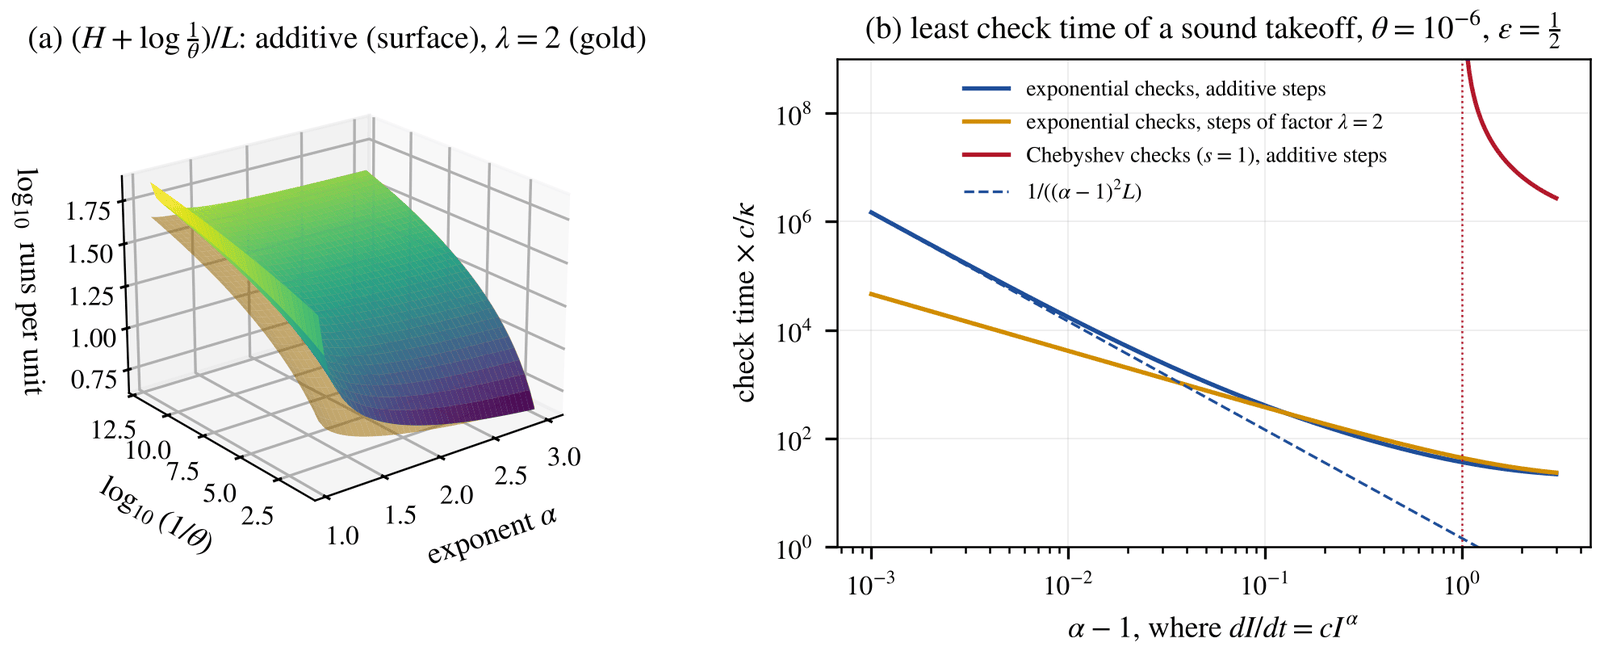
\includegraphics[width=0.98\textwidth]{figures/fig_takeoff}
\caption{Proposition~\ref{prop:osgood}, with $\eps=\frac12$. (a) The lower bound $(H+\log\frac1\theta)/L$ for the number of runs per unit of check cost, on a logarithmic scale, as a function of the growth exponent $\alpha$ and of $\log_{10}(1/\theta)$, for additive steps (coloured surface) and for doublings, $\lambda=2$ (gold surface). The additive surface rises like $1/(\alpha-1)$ as $\alpha\to1$, the multiplicative one like $\log\frac1{\alpha-1}$. (b) The lower bound for the least check time of a sound takeoff, in units of $\kappa/c$, at $\theta=10^{-6}$, against $\alpha-1$ on logarithmic axes: exponential checks with additive steps (blue), which approach $1/((\alpha-1)^{2}L)$ (dashed), exponential checks with doublings (gold), and Chebyshev checks with additive steps (red), which cost infinitely much for $\alpha\le2$ (dotted line).}
\label{fig:takeoff}
\end{figure*}

\subsection{What the growth exponent is, and what it is not}

The exponent $\alpha$ of Proposition~\ref{prop:osgood} is the elasticity of the speed of research with respect to the capability of the system that does it. It is not one of the exponents of the empirical scaling laws of language models. Kaplan and coauthors fitted the test loss of a language model trained with the optimal allocation of a compute budget $C$ to a power law $C^{-\alpha_{C}}$ with $\alpha_{C}\approx0.050$ \cite{KMH20}, and Hoffmann and coauthors fitted the loss as $E+A_{0}N^{-0.34}+B_{0}D^{-0.28}$ in the number $N$ of parameters and the number $D$ of training tokens \cite{HBM22}.\footnote{J.~Kaplan, S.~McCandlish, T.~Henighan, T.~B. Brown, B.~Chess, R.~Child, S.~Gray, A.~Radford, J.~Wu and D.~Amodei, \emph{Scaling laws for neural language models}, arXiv:2001.08361 (2020) \cite{KMH20}; J.~Hoffmann et~al., \emph{Training compute-optimal large language models}, arXiv:2203.15556 (2022) \cite{HBM22}. Both fits measure the cross-entropy loss on held-out text. The exponent $\alpha_{C}\approx0.050$ is that of the compute-efficient frontier in the first paper; the exponents $0.34$ and $0.28$, with fitted constants $E\approx1.69$, $A_{0}\approx406.4$ and $B_{0}\approx410.7$, are those of the parametric fit of the second. The letters $A_{0}$ and $B_{0}$ are renamed here to avoid a clash with the total cost $A$.} These laws relate loss to resources. To turn them into a value of $\alpha$ one needs two further maps, from loss to research ability and from research ability to the speed of the next improvement, and neither has been measured. Anbar Jafari, Ozcinar and Anbarjafari propose to estimate how fast improvement accelerates relative to its current level from series that engineers already record, which is an estimate of $\alpha$ \cite{AOA25}; the phase transitions and predictability limits of the first author with Singha Roy and Samal are a second approach to the same question \cite{BSS26}.

Ord observes that a singular growth path needs the generation time, the time around the loop of improvement, to tend to zero \cite{Ord26}. In the present model this is the condition $g_{n}\to0$, which a convergent $\sum g_{n}$ forces. Theorem~\ref{thm:E} adds a second clock: the time spent checking the $n$-th improvement must also tend to zero, and faster than the generation time can afford to, because the sum of $a_{n}\log(1/a_{n})$, and not only of $a_{n}$, must converge. Proposition~\ref{prop:osgood} shows that for power laws this second condition is free in kind and expensive in amount: every Osgood takeoff with $\alpha>1$ can be made sound with exponential checks, but near the threshold the checks take longer than the improvements by a factor that diverges as $1/(\alpha-1)$ when every unit of capability is checked. With checks that are only polynomially reliable, the threshold for a sound takeoff moves from $\alpha=1$ to $\alpha=1+s$, and between the two lies a range of singular takeoffs that cannot be made sound at any cost.

\begin{remark}[Errors of the generator]
Proposition~\ref{prop:osgood} prices the run in which every candidate is correct. If the $n$-th candidate is incorrect with probability in $[\rho_{\ast},\bar\rho]\subset(0,1)$ and incorrect candidates are regenerated, the proof of Theorem~\ref{thm:B}, with Proposition~\ref{prop:infinite} in place of Theorem~\ref{thm:A}, applies to the infinite chain: the lower bound holds with $\theta$ replaced by $\theta/\rho_{\ast}$, and the upper bound with $\theta$ replaced by $\theta(1-\bar\rho)/\bar\rho$ and the whole multiplied by $1/(1-\bar\rho)$. The orders in $\alpha-1$ of parts (ii) and (iii) do not change.
\end{remark}
